\chapter{Methodology}
This chapter details the methods used and the process with which we achieved our results.

\section{Process Overview} %Introductory chapter, sort of

\subsection{Exercise Description}
The goal of this exercise was to write a program for the EFM32GG that generated sounds by utilizing the onboard Digital to Analog Converter. The program should make at least three different sound effects, as well as a melody. These should be appropriate for use in the final exercise of the course where the goal is to create a game, and it should be possible to control which sound is being played by pressing the different buttons of the prototype gamepad. The program should be written in C, and should run directly on the EFM32GG hardware with no operating system involved. Emphasis was placed upon energy efficiency, an energy efficient solution will be rewarded with extra points.

TODO % Write something about the rest of the approach


\section{Initial Approach}
In order to get an introduction to programming the DAC we created a program intended to play a single continuous note. This would be an easy introduction to C programming, and would give us a good performance baseline with regards to energy consumption.

\subsection{GPIO Setup} 
The first step was porting the assembly code we had previosuly written to control LEDs and clocks over to C. Having set up the LEDs and buttons would also make it easier to debug the code by writing values to the LEDs to discern the current program state. Rather than starting with a simple polling loop we felt confident enough to go straight to interrupts for the LEDs and buttons, letting the program idle in a loop between interrupts.

The code we used to set up the GPIO pins for input and output is shown in code listing \ref{lst:gpio-setup1} and \ref{lst:gpio-setup2} respectively. In addition to the steps shown, the clock signal for the modules needed to be enabled in the CMU. \\

\noindent\begin{minipage}[pos=c,contentpos=c]{\textwidth}
  \begin{lstlisting}[caption=Setting GPIO pins 0-7 as input,label={lst:gpio-setup1}]
  *GPIO_PC_MODEL = 0x33333333;  // Set pins 0-7 as input pins
  *GPIO_PC_DOUT = 0xff;         // Enable pull-up resistors
  *GPIO_EXTIPSELL = 0x22222222; // Set interrupt generation for pin 0-7
  *GPIO_EXTIFALL = 0xff;        // Set interrupt on 1->0
  *GPIO_EXTIRISE = 0xff;        // Set interrupt on 0->1
  *GPIO_IEN = 0xff;             // Enable interrupt generation
  \end{lstlisting}
\end{minipage}

\noindent\begin{minipage}[c]{\textwidth}
  \begin{lstlisting}[caption=Setting GPIO pins 8-15 as output,label={lst:gpio-setup2}]
  *GPIO_PA_MODEH = 0x55555555; // Set pins 8-15 to output
  *GPIO_PA_CTRL = 2;           // Set high drive strength
  \end{lstlisting}
\end{minipage}


\subsection{DAC Setup}
The setup code we wrote for the DAC closely followed the instructions in the compendium, as shown in code listing \ref{lst:dac-setup}. With this setup, the DAC would continuously read both its 12 bit channels and update the output voltage. The next step to generate sound was to continously write samples to the channels emulating an audible waveform.\\

\noindent\begin{minipage}[c]{\textwidth}
  \begin{lstlisting}[caption=Setting up the DAC,label={lst:dac-setup}]
  *DAC0_CTRL = 0x50000; // Set a DAC clock division factor of 32
  *DAC0_CTRL |= 0x10;   // Set continuous mode
  *DAC0_CH0CTRL = 1;    // Enable left channel
  *DAC0_CH1CTRL = 1;    // Enable right channel
  \end{lstlisting}
\end{minipage}

\subsection{TIMER setup}
We chose to base our initial implementation on interrupts, writing a new sample to the DAC whenever an interrupt occurred. The sampling rate could then be set by setting the frequency of the interrupts. To generate interrupts, we used the TIMER module, setup as described in listing \ref{lst:timer-setup}. Note the variable \texttt{period} used to set interrupt frequency. \\

\noindent\begin{minipage}[c]{\textwidth}
  \begin{lstlisting}[caption=Setting up the timer to generate interrupts,label={lst:timer-setup}]
  *TIMER1_TOP = period; // Set period between interrupts
  *TIMER1_IEN = 1;      // Enable interrupt generation
  *TIMER1_CMD = 1;      // Start the timer
  \end{lstlisting}
\end{minipage}

Finally, an interrupt handler was written that used a simple conditional statement to write a square waveform to the DAC channels, oscillating the DAC voltage between 0 and 1000. Our first attempt was outside of the audible frequency range, but by adjusting the timer we could reduce the amount of interrupts to control the frequency.


\section{Efficient Interrupts}
After setting up everything we needed to generate a simple tone we decided to do some preliminary optimizations in our program. Rather than using the TIMER module we would use the LETIMER with a max speed of 32678 Hz, more than ample for our needs. As the LETIMER module was available in EM2 and EM3, this would allow us to potentially save energy by entering EM2 between the interrupts. \\

% and turning off the HF clock between samples.

\subsection{LETIMER and LFACLK Setup}
As the LETIMER is driven by the LFACLK clock, we needed to configure the LFACLK clock before using the LETIMER. The LFACLK was configured using the code shown in listing \ref{lst:lfaclk-setup}, and the LETIMER was configured using the code shown in listing \ref{lst:letimer-setup}. 

\subsubsection{Choosing Low Frequency Oscillator}
To drive the LFACLK we had the choice of either using the Low Frequency Crystal Oscillator (LFXO) or the Low Frequency RC Oscillator (LFRCO). After some initial testing we found that the LFRCO was unstable due to temperature differences, producing a slight variation in the pitch of the generated sound. LFXO was stable enough for our purposes. However, it had a longer start-up time, and we were aware that it might introduce delays into our program when waking up from low energy modes. \cite{efm32-oscillator-design-considerations-application-note} \\
 
\noindent\begin{minipage}[c]{\textwidth}
  \begin{lstlisting}[caption=Setting up the LFACLK to drive the LETIMER ,label={lst:lfaclk-setup}]
  *CMU_OSCENCMD |= (1 << 8);    // Start the LFXO
  *CMU_LFCLKSEL &= ~(0x3 << 0); // Select LFXO to drive LFACLK
  *CMU_LFCLKSEL |= (2 << 0);    //
  *CMU_LFACLKEN0 |= (1 << 2);   // Enable clock signal for LETIMER 

  // Enable clock for the Low Energy Peripheral Interface
  *CMU_HFCORECLKEN0 |= (1 << 4);
  \end{lstlisting}
\end{minipage}

\noindent\begin{minipage}[c]{\textwidth}
  \begin{lstlisting}[caption=Setting up LETIMER to generate periodic interrupts,label={lst:letimer-setup}]
  *LETIMER0_CTRL |= (1 << 9); // Set period between interrupts
  *LETIMER0_COMP0 = period;   // 
  *LETIMER0_CMD |= (1 << 0);  // Start the LETIMER
  *LETIMER0_IEN |= (1 << 2);  // Enable interrupt generation
  \end{lstlisting}
\end{minipage}


\section{Generating Songs}
We decided early in the process that we wanted to use the EFM32GG to play songs. We explored several different methods to create songs with the EFM32GG, and eventually decided on two different approaches. In the first approach, pre-synthesized samples were loaded on to the board at compile time. In the second approach, distinct notes coded as 16 bits words were loaded on to the board at compile time, and then synthesized at run-time by a software synthesizer. The result was two different implementations: The \emph{on-board synthesizer} and the \emph{sample-based music player}, described in section \ref{sec:onboard-synthesizer} and \ref{sec:sample-based-music-player} respectively.

\subsection{Memory Limitations}
The EFM32GG board has 128 kB of SRAM and 1024 kB of flash memory. This puts limitations on how a song is stored in the memory on the EFM32GG. Considering stoting the samples of a song sampled at 44100 Hz where each individual sample is 2 bytes large and the song duration is $d$ seconds. The size of the song can be calculated with the formula
$$\text{Song size (bytes)} = 88.2 \cdot d$$.
To find the longest song with a size that will fit in SRAM, we set $88200d = 128 kB = 131072 B$ which yields $d = 1.49$. Thus the longest song that will fit in SRAM is shorter than 1.5 seconds! This can be remedied somewhat by choosing a lower sample rate and possibly utilizing flash memory, but the EFM32GG will be hard pressed to store any quality song much longer than 30 seconds. Our two approaches uses different techniques to evade the memory limitations.

\subsection{On-board Synthesizer}\label{sec:onboard-synthesizer}
To overcome the memory limitations, this implementation uses the EFM32GG as a synthesizer to generate square waveforms. A song is stored in memory as integer arrays. The integer array contains information to create different tones. Two integer arrays produces a song with two channels.

Our first thought was to save all the samples of a song. 

\subsubsection{Song Representation}
In our solution we chose to represent a song as an array of 16 bit int values. These arrays is generated by a python script and placed in the source code. Inside these 16 bits we store information about pitch, octave, amplitude and duration. In table \ref{tab:bitFields} the bit partitions are described.

\begin{table}[H]
	\begin{center}
	\begin{tabular}{ |c|c|c|c| }
	  \hline
	  Duration & Amplitude & Octave & Pitch \\
	  \hline
	  5 & 3 & 4 & 4 \\
	  \hline

	\end{tabular}
	\caption{Bit partitioning}
	\label{tab:bitFields}
	\end{center}
\end{table}

Each pitch value is represented by a value from 0 to 11. The Octave can take the values 0-10. Note A with octave 0 is lowest possible at 27.5 Hz, and note A with octave 10 the highest at 28160 Hz. DAC's lowest values is to low hear, beacuse of this we calculated the amplitude with the equation \ref{eq:amplitudCalculation}. In addition we only had 3 bit to store the amplitude values, and as a result we calculated it exponentially. Duration takes values between 0-32. In our program we define the duration of the shortest note. The duration value is multiplied with the defined duration value and returns each notes duration given in milliseconds. By changing the defined duration value we can increase or decrease the song's speed.

\begin{equation}
  x = 2^{amplitude + 5}
  \label{eq:amplitudCalculation}
\end{equation}

\subsubsection{Song Playback}
To play a song the synthesizer wakes up 32768 times every second. Each tone is played with square waves. After calculating each tone's frequency the synthesizer turns the DAC on and off, to match the tone frequency. This method has limitations when it comes to reproducing sounds, but this metod is very space efficient.


\subsection{Sample Based Music Player}\label{sec:sample-based-music-player}
An issue with the synth is that in order to generate more advanced waveforms a program must utilize expensive trigonometric calculations to express them. Although the EFM32GG does have the capability to generate a sine wave on the DAC, in order to play actual music a more advance approach is required. To achieve this we decided to do the expensive calculations on a personal computer, using a synthesizer to sample a sine wave and output an array that could be compiled. Although the limited DAC sound quality made it possible to use a fairly low sample rate with no discernable quality difference we settled on using the maximum sample rate the LFXO clock could grant us, 32768 samples per second. 

\subsubsection{Song Representation}
In order to play back sound at a given sample S with B bits accuracy the required data is S*B per second. for 12 bits accuracy at a 32768 samples per second that equates 48kB for a second of music, unfeasible for the 128kB of SRAM the EFM32GG has. Additionally, in order to simplify access to sample the 12 bit values would be loaded into 2 bytes, effectively making each 12 bit sample take 16 bits of storage. In order to save space we therefore decided to create samples of the frequencies we needed into short segments that could be repeated as long as we wanted the sound to play. To implement this idea we created an array with 100 sample pointers as a lookup table for notes, where every note was assigned its own number, initializing only the pointers that pointed to a note that would be played. A song could then be encoded as an array of instructions to access various notes and repeat the sample for a set duration.


\begin{figure}[ht]
  \centering
  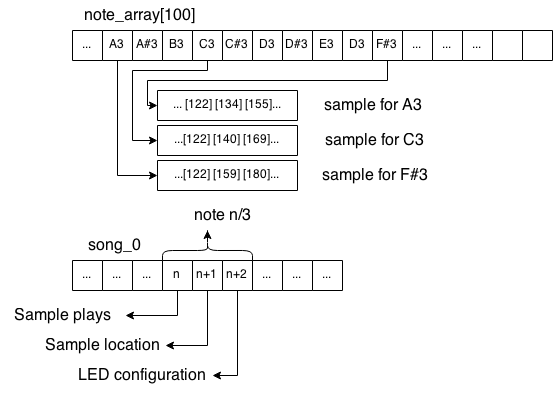
\includegraphics[width=\textwidth]{images/sample_array_layout.png}
  \caption{A map of the memory layout for the sample based approach}\label{fig:array_layout}
\end{figure}

\begin{minipage}{\textwidth}
\begin{lstlisting}
typedef struct Player
{
	uint16_t song;			// Number of current song
	uint16_t song_len;		// Total notes for current song
	uint16_t notes_played;	// Keeps track of notes
	uint16_t sample_total;	// Times current sample should play	
	uint16_t sample;		// Times current sample has played
	uint16_t sample_i;		// Position in current sample 
	uint16_t note_len;		// Length of current sample
	uint16_t* note;			// Location of current sample
	uint16_t LED;			// Current LED configuration
} Player;
\end{lstlisting}
\end{minipage}

\subsubsection{Song Playback}
In order to play a song we bundled the necessary attributes to keep track of what notes to play and their tempo together in a Play struct. To initialize a song play\_init() is called with the song to be played as the argument. This sets up a playback. After initializing calling the play() function will output the next sample to the DAC.
The play() function keeps track on the current position of a playback, reading from an array of triplets to load the next note whenever the current one has been finished.

\begin{minipage}{\textwidth}
\begin{lstlisting}
void play(void){
	// Load the next sample
	if(player.sample_i < player.note_len-1){			
		player.sample_i++;								
	}
	else{								
		player.sample_i = 0;
		if(player.sample < player.sample_total){
   			player.sample++;				
		}
		else{							
			player.sample = 0;
			if(player.notes_played < player.song_len){
				next_note();
				(*GPIO_PA_DOUT) =  player.note_len << 8 ;		
			}			 
			else{
			  disableLETIMER();
			  disableDAC();
			  //__asm("wfi");
			}
		}
	}
	// Write the sample to the DAC
	*DAC0_CH0DATA = player.note[player.sample_i];
	*DAC0_CH1DATA = player.note[player.sample_i];
}
\end{lstlisting}
\end{minipage}



\section{Testing}
In order to test the functionality of our program we relied on visual and aural feedback rather than software approaches such as GDB. By using the LEDs we could write values directly to the LEDs, and with the earphones we could hear whether the sound was playing correctly or not. In order to measure energy consumption we used the onboard LCD screen for quick estimates. For more quality measurements we used eAProfiler on a PC to read energy consumption on the board via the USB connection. In order to get quality measurements we performed them all in succsession on a board that had been in use for several hours to minimize measurement variance. 

\section{Optimization}

% stuff
As a considerable energy reduction was achieved by entering by entering energy mode EM1 after writing samples to the DAC, it was natural to think that entering EM2 would lower the energy reduction even further. One issue that occurred while implementing this functionality, is that the TIMER used to generate interrupts for the microcontroller is only available in energy modes EM0 and EM1. Thus if the microcontroller is to enter EM2 or lower energy modes, a different source of interupts is needed. The EFM32GG implements this functionality with the LETIMER module introduced in section \ref{sec:letimer}.

% TODO: Put this section somewhere appropriate
% TODO: Write about how using interrupts to sleep between each sample written to the DAC saves energy
\subsection{Sleeping Between Interrupts}
During music playback the board recieves 32.768 interrupts each second. In the time between interrupts we placed the board in sleep mode. We tried different energy modes to measure the energy consumption and the result can bee seen in \ref{sec:energyModeResults}.
